%% METADATA
%% subject-code: 4311102
%% subject-name: Fundamentals of Electronics
%% semester: 1
%% examination: Summer-2024
%% date: 21-06-2024
%% description: Solution guide for Fundamentals of Electronics Summer 2024 exam
%% tags: study-material, solutions, gtu, 4311102, electronics, diploma
%% END METADATA

\documentclass{article}

% content/resources/templates/preamble.tex
\usepackage[margin=0.6in]{geometry}
\author{Milav Dabgar}
\usepackage{amsmath,amssymb,amsthm}
\usepackage{booktabs}
\usepackage{multirow}
\usepackage{xcolor}
\usepackage{tcolorbox}
\tcbuselibrary{breakable,skins}
\usepackage[colorlinks=true,linkcolor=blue]{hyperref}
\usepackage{titlesec}
\usepackage{enumitem}
\usepackage{tikz}
\usepackage{pgfplots}
\usepackage{circuitikz}
\usepackage[version=4]{mhchem}
\usepackage{longtable}
\usepackage{array}
\usepackage{float}
\usepackage{caption}
\usepackage{listings}

\lstset{
  basicstyle=\small\ttfamily,
  breaklines=true,
  breakatwhitespace=false,
  postbreak=\mbox{\textcolor{red}{$\hookrightarrow$}\space},
  float=false,
  numbers=left,
  numberstyle=\tiny\color{gray},
  numbersep=10pt,
  xleftmargin=2em,
  keywordstyle=\color{blue},
  commentstyle=\color{green!60!black},
  stringstyle=\color{purple},
  backgroundcolor=\color{gray!5},
  showstringspaces=false,
  tabsize=2,
  captionpos=b,
  keepspaces=true,
  columns=flexible
}

\pgfplotsset{compat=1.18}
\usetikzlibrary{shapes,arrows,positioning,calc,patterns,decorations.pathmorphing,decorations.markings,arrows.meta}

% Color scheme
\definecolor{headcolor}{RGB}{0,102,204}
\definecolor{keycolor}{RGB}{220,20,60}
\definecolor{solutioncolor}{RGB}{34,139,34}
\definecolor{mnemoniccolor}{RGB}{148,0,211}
\definecolor{codecolor}{RGB}{0,0,100}

% Spacing
\setlength{\parskip}{3pt}
\setlist[itemize]{nosep}
\setlist[enumerate]{nosep}

% Title formatting
\titleformat{\section}{\Large\bfseries\color{headcolor}}{\thesection}{1em}{}
\titleformat{\subsection}{\large\bfseries\color{headcolor}}{\thesubsection}{1em}{}

% Pandoc tightlist compatibility
\providecommand{\tightlist}{%
  \setlength{\itemsep}{0pt}\setlength{\parskip}{0pt}}

% Pandoc longtable compatibility
\newcounter{none}
\def\thenone{}

\usetikzlibrary{decorations.pathmorphing}

\title{Fundamentals of Electronics (4311102) - Summer 2024 Solution}
\date{June 21, 2024}

\hypersetup{
  pdftitle={Fundamentals of Electronics (4311102) - Summer 2024 Solution},
  pdfsubject={GTU Exam Solution - Summer 2024},
  pdfauthor={Milav Dabgar},
  pdfkeywords={study-material, solutions, gtu, 4311102, electronics, fundamentals},
  pdfcreator={xelatex}
}

\begin{document}
\maketitle

\setcounter{tocdepth}{5}
\tableofcontents
\newpage

% ========================================
% QUESTION 1: Short Answer Questions (Answer 7 out of 10)
% Total Marks: 14 (2 marks each)
% ========================================

\section{Question 1}
\textbf{Answer any SEVEN out of the following TEN questions (2 marks each):}

% ========================================
% Q1.1: Define Resistor and Unit
% ========================================

\subsection{Question 1.1 [2 marks]}
\textbf{Define resistor and give its unit.}

\subsubsection{Solution}

\paragraph{Definition:}
A \textbf{resistor} is a passive electrical component that opposes or restricts the flow of electric current in a circuit. It converts electrical energy into heat energy and is used to control current and voltage levels.

\paragraph{Unit:}
The SI unit of resistance is the \textbf{Ohm}, symbolized as \(\Omega\) (Greek letter Omega). One ohm is the resistance that allows one ampere of current to flow when one volt is applied across it.

Mathematically: \(R = \frac{V}{I}\) where \(V\) is voltage in volts and \(I\) is current in amperes.

\paragraph{Mnemonic:}
\emph{``Resistor Resists, measured in Ohms''!}

% ========================================
% Q1.2: Active and Passive Component Examples
% ========================================



\subsection{Question 1.2 [2 marks]}
\textbf{Give two examples of active and passive components each.}

\subsubsection{Solution}

\paragraph{Active Components:}
Components that can amplify signals and control electron flow by adding energy from external power source:
\begin{description}
    \item[Transistor:] Amplifies or switches electronic signals
    \item[Operational Amplifier (Op-Amp):] Performs mathematical operations on signals
\end{description}

\paragraph{Passive Components:}
Components that cannot amplify signals and only consume or store energy:
\begin{description}
    \item[Resistor:] Opposes current flow
    \item[Capacitor:] Stores energy in electric field
\end{description}

\begin{figure}[H]
\centering
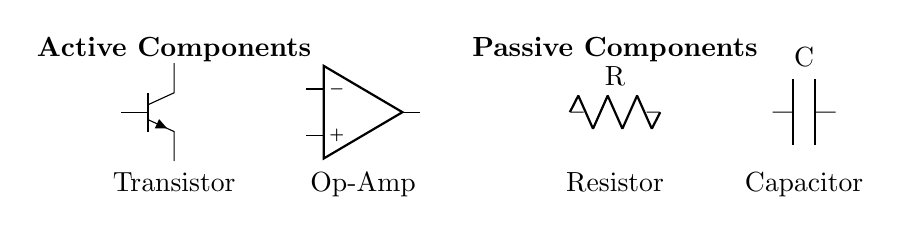
\begin{tikzpicture}[scale=0.8]
    % Active Components
    \node[font=\bfseries] at (0,3) {Active Components};

    % NPN Transistor
    \draw (0,2) node[npn, scale=0.8](npn1){};
    \node[below] at (0,1.2) {Transistor};

    % Op-Amp
    \draw (3,2) node[op amp, scale=0.6](opamp1){};
    \node[below] at (3,1.2) {Op-Amp};

    % Passive Components
    \node[font=\bfseries] at (7,3) {Passive Components};

    % Resistor
    \draw (6.5,2) to[R, l=R] (7.5,2);
    \node[below] at (7,1.2) {Resistor};

    % Capacitor
    \draw (9.5,2) to[C, l=C] (10.5,2);
    \node[below] at (10,1.2) {Capacitor};
\end{tikzpicture}
\caption{Examples of Active and Passive Components}
\end{figure}

\paragraph{Mnemonic:}
\emph{``Active Adds energy, Passive only Passes''!}

% ========================================
% Q1.3: Semiconductor Device Symbols
% ========================================



\subsection{Question 1.3 [2 marks]}
\textbf{Draw symbols of any two semiconductor devices.}

\subsubsection{Solution}

\begin{figure}[H]
\centering
\begin{circuitikz}[scale=1.2]
    % PN Junction Diode
    \draw (0,0) to[D, l=PN Diode] (2,0);
    \node[below] at (1,-0.5) {(a) PN Junction Diode};
    \node[left, font=\small] at (0,0) {Anode};
    \node[right, font=\small] at (2,0) {Cathode};

    % NPN Transistor
    \draw (5,0.5) node[npn, scale=1.2](npn){};
    \node at (npn.B) [left, font=\small] {Base};
    \node at (npn.C) [right, font=\small] {Collector};
    \node at (npn.E) [right, font=\small] {Emitter};
    \node[below] at (5,-0.8) {(b) NPN Transistor};
\end{circuitikz}
\caption{Semiconductor Device Symbols}
\end{figure}

\paragraph{Explanation:}
\begin{description}
    \item[PN Diode:] Triangle points in direction of conventional current flow (anode to cathode). Allows current in forward bias only.
    \item[NPN Transistor:] Arrow on emitter points outward (Not Pointing iN). Has three terminals: Base (control), Collector, and Emitter.
\end{description}

\paragraph{Mnemonic:}
\emph{``Diode arrow shows current Direction; NPN arrow points outwaNrd''!}

% ========================================
% Q1.4: Intrinsic vs Extrinsic Semiconductor
% ========================================



\subsection{Question 1.4 [2 marks]}
\textbf{Differentiate between intrinsic and extrinsic semiconductor.}

\subsubsection{Solution}

\begin{table}[H]
\centering
\caption{Intrinsic vs Extrinsic Semiconductor}
\begin{tabularx}{\textwidth}{lXX}
\toprule
\textbf{Parameter} & \textbf{Intrinsic} & \textbf{Extrinsic} \\
\midrule
Purity & Pure semiconductor (Si, Ge) & Doped with impurities \\
Conductivity & Low & Higher than intrinsic \\
Charge Carriers & \(n = p\) (equal) & \(n \neq p\) (unequal) \\
Temperature Effect & Highly sensitive & Less sensitive \\
Doping & No impurities added & Trivalent/Pentavalent added \\
Example & Pure Silicon at room temp & P-type, N-type Si \\
\bottomrule
\end{tabularx}
\end{table}

\begin{figure}[H]
\centering
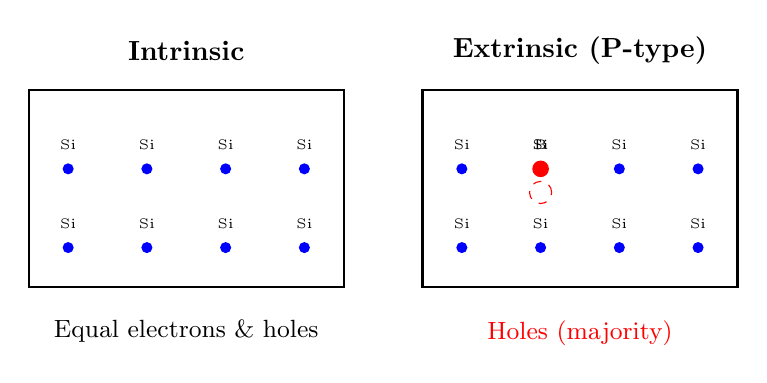
\begin{tikzpicture}[scale=1.0]
    % Intrinsic
    \node[font=\bfseries] at (2,3) {Intrinsic};
    \draw[thick] (0,0) rectangle (4,2.5);
    \foreach \x in {0.5,1.5,2.5,3.5} {
        \foreach \y in {0.5,1.5} {
            \fill[blue] (\x,\y) circle (2pt);
            \node[font=\tiny] at (\x,\y+0.3) {Si};
        }
    }
    \node[below, font=\small] at (2,-0.3) {Equal electrons \& holes};

    % Extrinsic (P-type)
    \node[font=\bfseries] at (7,3) {Extrinsic (P-type)};
    \draw[thick] (5,0) rectangle (9,2.5);
    \foreach \x in {5.5,6.5,7.5,8.5} {
        \foreach \y in {0.5,1.5} {
            \fill[blue] (\x,\y) circle (2pt);
            \node[font=\tiny] at (\x,\y+0.3) {Si};
        }
    }
    \fill[red] (6.5,1.5) circle (3pt);
    \node[font=\tiny] at (6.5,1.8) {B};
    \draw[red, dashed] (6.5,1.2) circle (4pt);
    \node[below, font=\small, red] at (7,-0.3) {Holes (majority)};
\end{tikzpicture}
\caption{Intrinsic vs Extrinsic Semiconductor Structure}
\end{figure}

\paragraph{Mnemonic:}
\emph{``Intrinsic is pure Inside; Extrinsic has Extra impurities''!}

% ========================================
% Q1.5: LED Full Form
% ========================================



\subsection{Question 1.5 [2 marks]}
\textbf{LED stands for \_\_\_\_\_\_\_\_\_\_\_\_\_\_\_\_\_.}

\subsubsection{Solution}

\paragraph{Full Form:}
LED stands for \textbf{Light Emitting Diode}.

\paragraph{Explanation:}
It is a semiconductor device that emits light when current flows through it in forward bias direction. The light emission occurs due to electroluminescence - recombination of electrons and holes releases energy as photons.

\paragraph{Mnemonic:}
\emph{``LED: Light Emits when Diode conducts''!}

% ========================================
% Q1.6: Photo-diode Applications
% ========================================

\subsection{Question 1.6 [2 marks]}
\textbf{State any two applications of Photo-diode.}

\subsubsection{Solution}

\paragraph{Applications:}
\begin{enumerate}
    \item \textbf{Optical Communication:} Used as light detector in fiber optic systems to convert optical signals to electrical signals.
    \item \textbf{Automatic Light Control:} Used in street lights, cameras, and displays to detect ambient light levels and adjust brightness automatically.
\end{enumerate}

\paragraph{Additional Applications:}
Light meters, barcode readers, smoke detectors, solar cells, infrared remote controls.


\paragraph{Note:} Photodiode always operates in reverse bias. It converts light energy into electrical energy. In industries, it is used in security systems.
\paragraph{Mnemonic:}
\emph{``Photo-diode detects Photons, converts to current''!}

% ========================================
% Q1.7: Transistor Types and Symbols
% ========================================

\subsection{Question 1.7 [2 marks]}
\textbf{List the types of transistor and draw their symbols.}

\subsubsection{Solution}

\paragraph{Types of Transistors:}
\begin{description}
    \item[BJT (Bipolar Junction Transistor):] NPN and PNP types
    \item[FET (Field Effect Transistor):] JFET and MOSFET types
\end{description}

\begin{figure}[H]
\centering
\begin{circuitikz}[scale=1.1]
    % NPN
    \node[font=\bfseries] at (1.5,3) {BJT Types};
    \draw (0,1.5) node[npn, scale=1.1](npn){};
    \node at (npn.B) [left, font=\small] {B};
    \node at (npn.C) [above right, font=\small] {C};
    \node at (npn.E) [below right, font=\small] {E};
    \node[below] at (0,0.2) {NPN};

    % PNP
    \draw (3,1.5) node[pnp, scale=1.1](pnp){};
    \node at (pnp.B) [left, font=\small] {B};
    \node at (pnp.C) [below right, font=\small] {C};
    \node at (pnp.E) [above right, font=\small] {E};
    \node[below] at (3,0.2) {PNP};

    % N-channel JFET
    \node[font=\bfseries] at (7.5,3) {FET Types};
    \draw (6,1.5) node[njfet, scale=1.1](njfet){};
    \node at (njfet.G) [left, font=\small] {G};
    \node at (njfet.D) [above right, font=\small] {D};
    \node at (njfet.S) [below right, font=\small] {S};
    \node[below] at (6,0.2) {N-JFET};

    % N-channel MOSFET
    \draw (9,1.5) node[nmos, scale=1.1](nmos){};
    \node at (nmos.G) [left, font=\small] {G};
    \node at (nmos.D) [above right, font=\small] {D};
    \node at (nmos.S) [below right, font=\small] {S};
    \node[below] at (9,0.2) {N-MOSFET};
\end{circuitikz}
\caption{Transistor Types and Their Symbols}
\end{figure}


\paragraph{Remember:} BJT is a current controlled device while FET is a voltage controlled device. Both are used for amplification and switching.
\paragraph{Mnemonic:}
\emph{``NPN: Not Pointing iN; PNP: Pointing iN Please''!}

% ========================================
% Q1.8: Ge and Si Forward Voltage Drop
% ========================================

\subsection{Question 1.8 [2 marks]}
\textbf{Give the value of forward voltage drop of Germanium and Silicon diode.}

\subsubsection{Solution}

\paragraph{Forward Voltage Drop Values:}
\begin{description}
    \item[Germanium (Ge) Diode:] \(V_f \approx 0.3\,V\)  
    \item[Silicon (Si) Diode:] \(V_f \approx 0.7\,V\)
\end{description}

\paragraph{Explanation:}
Forward voltage drop is the minimum voltage required across a diode for it to conduct in forward bias. Silicon has higher bandgap energy (\(1.1\,eV\)) than Germanium (\(0.7\,eV\)), hence requires more voltage to overcome barrier potential.

\paragraph{Comparison:}
Si diodes are more commonly used due to better temperature stability and lower reverse leakage current, despite higher forward drop.


\paragraph{Difference:} Silicon (Si) is used more because it remains stable at higher temperatures. Germanium (Ge) has higher leakage current.
\paragraph{Mnemonic:}
\emph{``Silicon Seven-tenths (0.7V); Germanium three-tenths (0.3V)''!}

% ========================================
% Q1.9: Photo-diode as Light Detector (Fill in Blank)
% ========================================

\subsection{Question 1.9 [2 marks]}
\textbf{The \_\_\_\_\_\_\_\_\_\_\_\_\_\_\_\_\_ diode can be used as a light detector.}

\subsubsection{Solution}

\paragraph{Answer:}
The \textbf{Photo} diode (or \textbf{Photodiode}) can be used as a light detector.

\paragraph{Explanation:}
A photodiode operates in reverse bias and generates current proportional to the intensity of light falling on it. When photons strike the PN junction, they create electron-hole pairs, producing photocurrent.


\paragraph{Reason:} When light falls on the photodiode, minority carriers are generated, increasing reverse current. This principle is used for light detection.
\paragraph{Mnemonic:}
\emph{``Photo-diode for Photos (light detection)''!}

% ========================================
% Q1.10: Q-Factor of Coil
% ========================================

\subsection{Question 1.10 [2 marks]}
\textbf{Define Q-factor of a coil.}

\subsubsection{Solution}

\paragraph{Definition:}
The \textbf{Quality factor (Q-factor)} of a coil is a dimensionless parameter that represents the ratio of its inductive reactance to its resistance at a particular frequency. It indicates how ``pure'' or ``ideal'' the inductor is.

\paragraph{Formula:}
\[
Q = \frac{X_L}{R} = \frac{\omega L}{R} = \frac{2\pi f L}{R}
\]

where \(X_L\) is inductive reactance, \(R\) is coil resistance, \(L\) is inductance, and \(f\) is frequency.

\paragraph{Significance:}
Higher Q-factor means lower energy loss, sharper resonance in tuned circuits, and better selectivity in RF applications. Typical values range from 10 to 100+ for good coils.


\paragraph{Importance:} High Q-factor means the circuit is more selective and bandwidth is narrow. Q-factor is a very important parameter in resonant circuits.
\paragraph{Mnemonic:}
\emph{``Q is Quality: reactance over resistance''!}

% ========================================
% QUESTION 2: Components & Properties (14 marks)
% Demonstrates: Component characteristics, EM induction, calculations
% ========================================




\section{Question 2}

% This section covers passive components and their properties.

% ========================================
% Q2(a): Color Coding Method [3 marks]
% ========================================


\subsection{Question 2(a) [3 marks]}
\textbf{Explain colour coding method of resistor.}

\subsubsection{Solution}

The \textbf{resistor color code} is a standardized system used to indicate the resistance value, tolerance, and sometimes temperature coefficient of resistors through colored bands painted on the resistor body.

\paragraph{Standard 4-Band Color Code:}

\begin{table}[H]
\centering
\caption{Resistor Color Code Table}
\begin{tabularx}{\textwidth}{lXXXX}
\toprule
\textbf{Color} & \textbf{Digit} & \textbf{Multiplier} & \textbf{Tolerance} & \textbf{Temp Coeff} \\
\midrule
Black   & 0 & \(\times 10^0\) & - & - \\
Brown   & 1 & \(\times 10^1\) & \(\pm 1\%\) & 100 ppm \\
Red     & 2 & \(\times 10^2\) & \(\pm 2\%\) & 50 ppm \\
Orange  & 3 & \(\times 10^3\) & - & 15 ppm \\
Yellow  & 4 & \(\times 10^4\) & - & 25 ppm \\
Green   & 5 & \(\times 10^5\) & \(\pm 0.5\%\) & - \\
Blue    & 6 & \(\times 10^6\) & \(\pm 0.25\%\) & 10 ppm \\
Violet  & 7 & \(\times 10^7\) & \(\pm 0.1\%\) & 5 ppm \\
Grey    & 8 & \(\times 10^8\) & - & - \\
White   & 9 & \(\times 10^9\) & - & - \\
Gold    & - & \(\times 0.1\) & \(\pm 5\%\) & - \\
Silver  & - & \(\times 0.01\) & \(\pm 10\%\) & - \\
\bottomrule
\end{tabularx}
\end{table}

\begin{figure}[H]
\centering
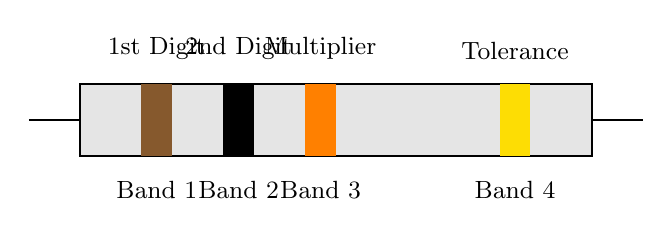
\begin{tikzpicture}[scale=1.3]
    % Resistor body
    \draw[thick, fill=gray!20] (0,0) rectangle (5,0.7);

    % Color bands
    \fill[brown!70!black] (0.6,0) rectangle (0.9,0.7);
    \fill[black] (1.4,0) rectangle (1.7,0.7);
    \fill[orange] (2.2,0) rectangle (2.5,0.7);
    \fill[yellow!80!orange] (4.1,0) rectangle (4.4,0.7);

    % Labels
    \node[below, font=\small] at (0.75,-0.15) {Band 1};
    \node[below, font=\small] at (1.55,-0.15) {Band 2};
    \node[below, font=\small] at (2.35,-0.15) {Band 3};
    \node[below, font=\small] at (4.25,-0.15) {Band 4};

    \node[above, font=\small] at (0.75,0.85) {1st Digit};
    \node[above, font=\small] at (1.55,0.85) {2nd Digit};
    \node[above, font=\small] at (2.35,0.85) {Multiplier};
    \node[above, font=\small] at (4.25,0.85) {Tolerance};

    % Leads
    \draw[thick] (-0.5,0.35) -- (0,0.35);
    \draw[thick] (5,0.35) -- (5.5,0.35);
\end{tikzpicture}
\caption{4-Band Resistor Color Code Structure}
\end{figure}

\paragraph{Reading Method:}
\begin{enumerate}
    \item Identify tolerance band (Gold/Silver, slightly separated) on RIGHT
    \item Read from LEFT to RIGHT
    \item Bands 1 \& 2: Significant digits
    \item Band 3: Multiplier (number of zeros)
    \item Band 4: Tolerance
\end{enumerate}

\paragraph{Example:}
Brown-Black-Orange-Gold = 1, 0, \(\times 10^3\), \(\pm 5\%\) = \(10{,}000\,\Omega \pm 5\%\) = \(10\,k\Omega \pm 5\%\)


\paragraph{Tip:} Use the `BBROYGBVGW' mnemonic to remember color codes. The Tolerance band should always be counted last.
\paragraph{Mnemonic:}
\emph{``BB ROY Great Britain Very Good Wife'' - Black Brown Red Orange Yellow Green Blue Violet Grey White!}

% ========================================
% Q2(a) OR: LDR with Characteristics [3 marks]
% ========================================

\subsection{Question 2(a) OR [3 marks]}
\textbf{Explain Light Dependent Resistor with its characteristics.}

\subsubsection{Solution}

A \textbf{Light Dependent Resistor (LDR)} or photoresistor is a passive component whose resistance varies inversely with the intensity of incident light.

\paragraph{Construction:}

\begin{figure}[H]
\centering
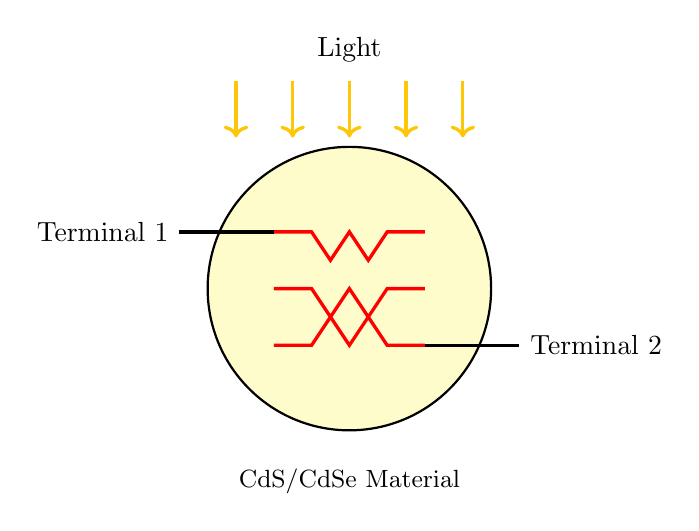
\begin{tikzpicture}[scale=1.2]
    % LDR body
    \draw[thick, fill=yellow!20] (0,0) circle (1.5);

    % Zigzag pattern (photoresistive material)
    \draw[very thick, red] 
        (-0.8,0.6) -- (-0.4,0.6) -- (-0.2,0.3) -- (0,0.6) -- (0.2,0.3) -- (0.4,0.6) -- (0.8,0.6);
    \draw[very thick, red]
        (-0.8,0) -- (-0.4,0) -- (-0.2,-0.3) -- (0,0) -- (0.2,-0.3) -- (0.4,0) -- (0.8,0);
    \draw[very thick, red]
        (-0.8,-0.6) -- (-0.4,-0.6) -- (-0.2,-0.3) -- (0,-0.6) -- (0.2,-0.3) -- (0.4,-0.6) -- (0.8,-0.6);

    % Terminals
    \draw[very thick] (-0.8,0.6) -- (-1.8,0.6) node[left] {Terminal 1};
    \draw[very thick] (0.8,-0.6) -- (1.8,-0.6) node[right] {Terminal 2};

    % Light rays
    \foreach \x in {-1.2,-0.6,0,0.6,1.2} {
        \draw[->, yellow!60!orange, very thick] (\x,2.2) -- (\x,1.6);
    }
    \node[above] at (0,2.3) {Light};

    % Labels
    \node[below, font=\small] at (0,-1.8) {CdS/CdSe Material};
\end{tikzpicture}
\caption{LDR Construction}
\end{figure}

\paragraph{Working Principle:}
Based on photoconductivity - when light photons strike the semiconductor material (CdS/CdSe), they impart energy to electrons, creating electron-hole pairs. This increases conductivity and decreases resistance.

\paragraph{Characteristics:}

\begin{figure}[H]
\centering
\begin{tikzpicture}[scale=1.0]
    % Axes
    \draw[->, thick] (0,0) -- (7,0) node[right] {Light Intensity (lux)};
    \draw[->, thick] (0,0) -- (0,5) node[above] {Resistance (k\(\Omega\))};

    % Characteristic curve (inverse relationship)
    \draw[blue, very thick, domain=0.3:6.5] plot (\x, {4.5/(\x+0.2)});

    % Points
    \fill[red] (1,3.8) circle (2pt) node[right, font=\small] {Dark: \(\sim\)1M\(\Omega\)};
    \fill[red] (6,0.72) circle (2pt) node[above right, font=\small] {Bright: \(\sim\)100\(\Omega\)};

    % Grid lines
    \draw[dashed, gray] (0,3.8) -- (1,3.8);
    \draw[dashed, gray] (0,0.72) -- (6,0.72);
\end{tikzpicture}
\caption{LDR Resistance vs Light Intensity Characteristic}
\end{figure}

\paragraph{Specifications:}
\begin{itemize}
    \item Dark Resistance: 1M\(\Omega\) - 10M\(\Omega\)
    \item Light Resistance: 100\(\Omega\) - 1k\(\Omega\)
    \item Response Time: 10-100ms
    \item Peak Spectral Response: ~550nm (green light)
\end{itemize}

\paragraph{Applications:}
Street lights, camera exposure control, alarm systems, light meters.


\paragraph{Tip:} Use the `BBROYGBVGW' mnemonic to remember color codes. The Tolerance band should always be counted last.
\paragraph{Mnemonic:}
\emph{``LDR: Light Down, Resistance Down''!}

% ========================================
% Q2(b): Capacitor Classification [3 marks]
% ========================================

\subsection{Question 2(b) [3 marks]}
\textbf{Explain classification of capacitors in detail.}

\subsubsection{Solution}

Capacitors are classified based on dielectric material, polarity, and construction.

\paragraph{Classification by Dielectric Material:}

\begin{description}
    \item[Ceramic Capacitors:] Use ceramic dielectric (barium titanate). Small, inexpensive, non-polarized. Values: pF to few \(\mu\)F.

    \item[Film Capacitors:] Plastic film dielectric (polyester, polypropylene). Stable, low loss. Values: nF to \(\mu\)F range.

    \item[Electrolytic Capacitors:] Aluminum oxide dielectric, polarized. High capacitance (1\(\mu\)F to 10000\(\mu\)F), used in power supplies.

    \item[Tantalum Capacitors:] Tantalum pentoxide dielectric, polarized. Stable, compact, expensive. Values: 0.1\(\mu\)F to 100\(\mu\)F.

    \item[Mica Capacitors:] Mica dielectric. Very stable, low loss, expensive. RF applications.
\end{description}

\begin{figure}[H]
\centering
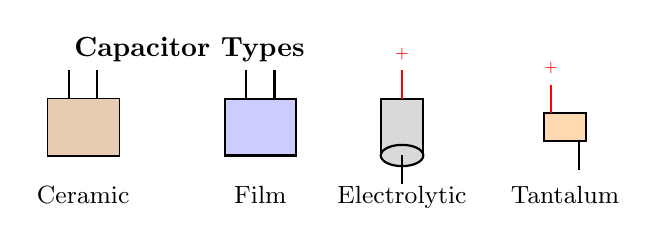
\begin{tikzpicture}[scale=0.9]
    % Ceramic
    \node[font=\bfseries] at (2,3.5) {Capacitor Types};
    \draw[thick] (0,2) rectangle (1,2.8);
    \fill[brown!40] (0,2) rectangle (1,2.8);
    \node[below, font=\small] at (0.5,1.7) {Ceramic};
    \draw[thick] (0.3,2.8) -- (0.3,3.2);
    \draw[thick] (0.7,2.8) -- (0.7,3.2);

    % Film
    \draw[thick, fill=blue!20] (2.5,2) -- (3.5,2) -- (3.5,2.8) -- (2.5,2.8) -- cycle;
    \node[below, font=\small] at (3,1.7) {Film};
    \draw[thick] (2.8,2.8) -- (2.8,3.2);
    \draw[thick] (3.2,2.8) -- (3.2,3.2);

    % Electrolytic (polarized)
    \draw[thick, fill=gray!30] (4.7,2) rectangle (5.3,2.8);
    \draw[thick, fill=gray!30] (5,2) ellipse (0.3 and 0.15);
    \node[below, font=\small] at (5,1.7) {Electrolytic};
    \draw[thick, red] (5,2.8) -- (5,3.2) node[above, font=\tiny] {+};
    \draw[thick] (5,2) -- (5,1.6);

    % Tantalum 
    \draw[thick, fill=orange!30] (7,2.2) rectangle (7.6,2.6);
    \node[below, font=\small] at (7.3,1.7) {Tantalum};
    \draw[thick, red] (7.1,2.6) -- (7.1,3.0) node[above, font=\tiny] {+};
    \draw[thick] (7.5,2.2) -- (7.5,1.8);
\end{tikzpicture}
\caption{Types of Capacitors}
\end{figure}

\paragraph{Classification by Polarity:}
\begin{description}
    \item[Polarized:] Must be connected with correct polarity (electrolytic, tantalum)
    \item[Non-Polarized:] Can be connected either way (ceramic, film, mica)
\end{description}


\paragraph{Property:} A capacitor blocks DC current and passes AC current.
\paragraph{Mnemonic:}
\emph{``CEFMT: Ceramic, Electrolytic, Film, Mica, Tantalum - Capacitor types''!}

% ========================================
% Q2(b) OR: Inductor Classification [3 marks]
% ========================================

\subsection{Question 2(b) OR [3 marks]}
\textbf{Explain classification of inductor in detail.}

\subsubsection{Solution}

Inductors are classified based on core material, construction, and application.

\paragraph{Classification by Core Material:}

\begin{description}
    \item[Air Core Inductors:] No magnetic core, just coiled wire. Low inductance (nH to \(\mu\)H), used in RF circuits. No core losses, no saturation.

    \item[Iron Core Inductors:] Solid iron core. High inductance, used in low-frequency applications. Heavy, subject to core losses.

    \item[Ferrite Core Inductors:] Ferrite (ceramic magnetic) core. Good for high-frequency switching applications. Lower losses than iron.

    \item[Powdered Iron Core:] Iron powder mixed with binder. Distributed air gap reduces saturation. Used in filters and RF chokes.

    \item[Laminated Core Inductors:] Thin iron sheets laminated together. Reduces eddy current losses. Used in transformers and power inductors.
\end{description}

\begin{figure}[H]
\centering
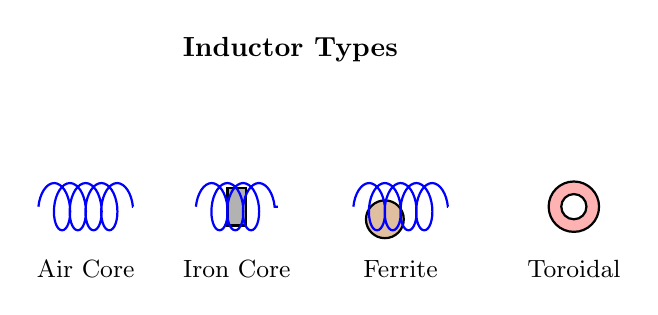
\begin{tikzpicture}[scale=0.8]
    % Air core
    \node[font=\bfseries] at (4,4) {Inductor Types};
    \draw[thick, blue, decoration={coil, aspect=0.5, segment length=2mm, amplitude=3mm}, decorate] (0,1.5) -- (1.5,1.5);
    \node[below, font=\small] at (0.75,0.8) {Air Core};

    % Iron core
    \draw[thick, fill=gray!60] (3,1.2) rectangle (3.3,1.8);
    \draw[thick, blue, decoration={coil, aspect=0.5, segment length=2mm, amplitude=3mm}, decorate] (2.5,1.5) -- (3.8,1.5);
    \node[below, font=\small] at (3.15,0.8) {Iron Core};

    % Ferrite core
    \draw[thick, fill=brown!50] (5.5,1.3) circle (0.3);
    \draw[thick, blue, decoration={coil, aspect=0.5, segment length=2mm, amplitude=3mm}, decorate] (5,1.5) -- (6.5,1.5);
    \node[below, font=\small] at (5.75,0.8) {Ferrite};

    % Toroidal
    \draw[thick, fill=red!30] (8.5,1.5) circle (0.4);
    \draw[thick, fill=white] (8.5,1.5) circle (0.2);
    \node[below, font=\small] at (8.5,0.8) {Toroidal};
\end{tikzpicture}
\caption{Types of Inductors by Core Material}
\end{figure}

\paragraph{Classification by Construction:}
\begin{description}
    \item[Solenoid:] Helical coil wound on cylindrical form
    \item[Toroidal:] Wire wound on donut-shaped core - self-shielding, compact
    \item[Multilayer:] Multiple layers of winding for high inductance
\end{description}

\paragraph{Mnemonic:}
\emph{``AIFPL: Air, Iron, Ferrite, Powdered, Laminated - Inductor cores''!}

% ========================================
% Q2(c): Faraday's Laws of EMI [4 marks]
% ========================================

\subsection{Question 2(c) [4 marks]}
\textbf{State and explain Faraday's laws of Electromagnetic Induction.}

\subsubsection{Solution}

Faraday's laws describe how a changing magnetic field induces an electromotive force (EMF) in a conductor.

\paragraph{First Law:}
\textbf{Statement:} Whenever the magnetic flux linking a conductor or coil changes, an EMF is induced in it.

\paragraph{Second Law:}
\textbf{Statement:} The magnitude of induced EMF is directly proportional to the rate of change of magnetic flux linkage.

\paragraph{Mathematical Expression:}
\[
\mathcal{E} = -N \frac{d\Phi}{dt}
\]

where:
\begin{itemize}
    \item \(\mathcal{E}\) = Induced EMF (volts)
    \item \(N\) = Number of turns
    \item \(\frac{d\Phi}{dt}\) = Rate of change of magnetic flux
    \item Negative sign indicates Lenz's Law (opposes the change)
\end{itemize}

\begin{figure}[H]
\centering
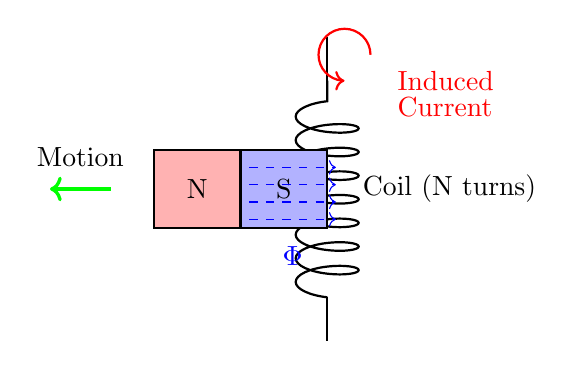
\begin{tikzpicture}[scale=1.1]
    % Coil
    \draw[thick] (0,0) -- (0,0.5);
    \draw[thick, decoration={coil, aspect=0.3, segment length=3mm, amplitude=4mm}, decorate] (0,0.5) -- (0,3);
    \draw[thick] (0,3) -- (0,3.5);
    \node[right] at (0.3,1.75) {Coil (N turns)};

    % Magnet moving
    \draw[thick, fill=red!30] (-2,1.3) rectangle (-1,2.2);
    \node at (-1.5,1.75) {N};
    \draw[thick, fill=blue!30] (-1,1.3) rectangle (0,2.2);
    \node at (-0.5,1.75) {S};
    \draw[->, very thick, green] (-2.5,1.75) -- (-3.2,1.75);
    \node[above] at (-2.85,1.9) {Motion};

    % Induced current
    \draw[->, thick, red] (0.5,3.3) arc (0:270:0.3);
    \node[right, red] at (0.7,3) {Induced};
    \node[right, red] at (0.7,2.7) {Current};

    % Flux lines
    \foreach \y in {1.4,1.6,1.8,2.0} {
        \draw[->, blue, dashed] (-0.9,\y) -- (0.1,\y);
    }
    \node[below, blue] at (-0.4,1.2) {\(\Phi\)};
\end{tikzpicture}
\caption{Electromagnetic Induction - Moving Magnet Induces EMF}
\end{figure}

\paragraph{Explanation:}
When a magnet moves toward/away from a coil, the magnetic flux through the coil changes. This changing flux induces an EMF that causes current to flow if the circuit is closed. The induced current creates its own magnetic field that opposes the original change (Lenz's Law).

\paragraph{Applications:}
Generators, transformers, inductors, induction motors, wireless charging.


\paragraph{Lenz's Law:} The induced EMF always opposes its cause.
\paragraph{Mnemonic:}
\emph{``Faraday: Flux change induces EMF, Rate determines magnitude''!}

% ========================================
% Q2(c) OR: Capacitor Specifications [4 marks]  
% ========================================




\subsection{Question 2(c) OR [4 marks]}
\textbf{Enlist specifications of capacitors and explain two in detail.}

\subsubsection{Solution}

\paragraph{Capacitor Specifications:}
\begin{enumerate}
    \item \textbf{Capacitance Value} (C)
    \item \textbf{Voltage Rating} (Working Voltage)
    \item \textbf{Tolerance}
    \item \textbf{Temperature Coefficient}
    \item \textbf{ESR (Equivalent Series Resistance)}
    \item \textbf{Leakage Current}
    \item \textbf{Ripple Current Rating}
    \item \textbf{Life Span / Endurance}
\end{enumerate}

\paragraph{Detailed Explanation:}

\subparagraph{1. Capacitance Value (C):}
The ability to store electric charge, measured in Farads (F). Practical units: pF (picofarad), nF (nanofarad), \(\mu\)F (microfarad).

Formula: \(C = \frac{Q}{V}\) where Q is charge in coulombs, V is voltage.

For parallel plate: \(C = \frac{\epsilon_0 \epsilon_r A}{d}\)

Typical ranges:
\begin{itemize}
    \item Ceramic: 1pF - 1\(\mu\)F
    \item Film: 1nF - 100\(\mu\)F
    \item Electrolytic: 1\(\mu\)F - 10000\(\mu\)F
\end{itemize}

\subparagraph{2. Voltage Rating (Working Voltage):}
Maximum DC voltage that can be continuously applied without breakdown. Exceeding this causes dielectric failure.

Derating: In practice, operate at 50-80\% of rated voltage for reliability.

Example ratings: 6.3V, 10V, 16V, 25V, 50V, 100V, 450V (common values)

\begin{description}
    \item[Safety Factor:] Always select voltage rating \(>\) 1.5 \(\times\) maximum circuit voltage
    \item[AC Applications:] Peak voltage must be less than DC rating
\end{description}

\paragraph{Mnemonic:}
\emph{``CV-TT-ELR-L: Capacitance, Voltage, Tolerance, Temperature, ESR, Leakage, Ripple, Life''!}

% ========================================
% Q2(d): Color Band for 47\(\Omega\)±5% [4 marks]
% ========================================

\subsection{Question 2(d) [4 marks]}
\textbf{Write colour band of 47\(\Omega\)±5\% resistance.}

\subsubsection{Solution}

For \textbf{47\(\Omega\) ±5\%} resistor using 4-band color code:

\paragraph{Calculation:}
\begin{itemize}
    \item Resistance = 47\(\Omega\) = 47 \(\times 10^0\)
    \item First digit = 4 → \textbf{Yellow}
    \item Second digit = 7 → \textbf{Violet}
    \item Multiplier = \(\times 10^0\) = \(\times 1\) → \textbf{Black}
    \item Tolerance = ±5\% → \textbf{Gold}
\end{itemize}

\paragraph{Color Band Sequence:}
\textbf{Yellow - Violet - Black - Gold}

\begin{figure}[H]
\centering
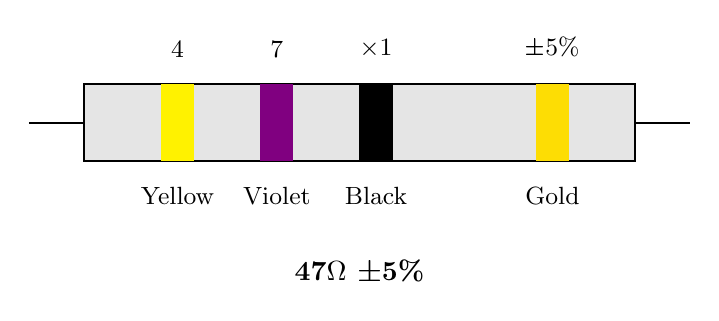
\begin{tikzpicture}[scale=1.4]
    % Resistor body
    \draw[thick, fill=gray!20] (0,0) rectangle (5,0.7);

    % Color bands
    \fill[yellow] (0.7,0) rectangle (1.0,0.7);
    \fill[violet] (1.6,0) rectangle (1.9,0.7);
    \fill[black] (2.5,0) rectangle (2.8,0.7);
    \fill[yellow!80!orange] (4.1,0) rectangle (4.4,0.7);

    % Labels
    \node[below, font=\small] at (0.85,-0.15) {Yellow};
    \node[below, font=\small] at (1.75,-0.15) {Violet};
    \node[below, font=\small] at (2.65,-0.15) {Black};
    \node[below, font=\small] at (4.25,-0.15) {Gold};

    \node[above, font=\small] at (0.85,0.85) {4};
    \node[above, font=\small] at (1.75,0.85) {7};
    \node[above, font=\small] at (2.65,0.85) {\(\times 1\)};
    \node[above, font=\small] at (4.25,0.85) {±5\%};

    % Leads
    \draw[thick] (-0.5,0.35) -- (0,0.35);
    \draw[thick] (5,0.35) -- (5.5,0.35);

    % Result
    \node[below, font=\bfseries] at (2.5,-0.8) {47\(\Omega\) ±5\%};
\end{tikzpicture}
\caption{47\(\Omega\) ±5\% Resistor Color Bands}
\end{figure}

\paragraph{Verification:}
Tolerance range: 47\(\Omega\) ± 5\% = 47 ± 2.35 = 44.65\(\Omega\) to 49.35\(\Omega\)


\paragraph{Importance:} The Tolerance band indicates the precision and quality of the resistor.
\paragraph{Mnemonic:}
\emph{``Yellow Violet Black Gold = 47 ohms, Five percent told''!}

% ========================================
% Q2(d) OR: Calculate Brown-Black-Yellow [4 marks]
% ========================================

\subsection{Question 2(d) OR [4 marks]}
\textbf{Calculate value of resistor and tolerance for a given colour code: Brown, Black, yellow.}

\subsubsection{Solution}

Given color code: \textbf{Brown - Black - Yellow}

\paragraph{Reading the Colors:}
\begin{itemize}
    \item Band 1 (Brown): First digit = \textbf{1}
    \item Band 2 (Black): Second digit = \textbf{0}
    \item Band 3 (Yellow): Multiplier = \textbf{\(\times 10^4\)}
    \item Band 4: Not given, assume \textbf{no tolerance band} or ±20\% (default for 3-band)
\end{itemize}

\paragraph{Calculation:}
\[
R = (10) \times 10^4 = 100{,}000\,\Omega = 100\,k\Omega
\]

\paragraph{Tolerance:}
Since only 3 bands are given, tolerance is typically ±20\% (standard for 3-band resistors).

\begin{figure}[H]
\centering
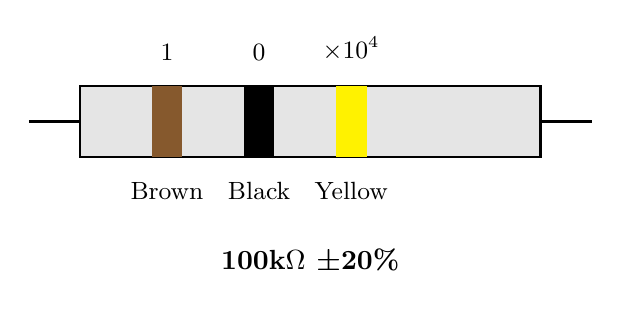
\begin{tikzpicture}[scale=1.3]
    % Resistor body
    \draw[thick, fill=gray!20] (0,0) rectangle (4.5,0.7);

    % Color bands  
    \fill[brown!70!black] (0.7,0) rectangle (1.0,0.7);
    \fill[black] (1.6,0) rectangle (1.9,0.7);
    \fill[yellow] (2.5,0) rectangle (2.8,0.7);

    % Labels
    \node[below, font=\small] at (0.85,-0.15) {Brown};
    \node[below, font=\small] at (1.75,-0.15) {Black};
    \node[below, font=\small] at (2.65,-0.15) {Yellow};

    \node[above, font=\small] at (0.85,0.85) {1};
    \node[above, font=\small] at (1.75,0.85) {0};
    \node[above, font=\small] at (2.65,0.85) {\(\times 10^4\)};

    % Leads
    \draw[thick] (-0.5,0.35) -- (0,0.35);
    \draw[thick] (4.5,0.35) -- (5,0.35);

    % Result
    \node[below, font=\bfseries] at (2.25,-0.8) {100k\(\Omega\) ±20\%};
\end{tikzpicture}
\caption{Brown-Black-Yellow = 100k\(\Omega\)}
\end{figure}

\paragraph{Tolerance Range:}
100k\(\Omega\) ± 20\% = 100k ± 20k = 80k\(\Omega\) to 120k\(\Omega\)

\paragraph{Answer:}
\begin{description}
    \item[Resistance:] \textbf{100 k\(\Omega\)}
    \item[Tolerance:] \textbf{±20\%} (80k\(\Omega\) - 120k\(\Omega\))
\end{description}

\paragraph{Mnemonic:}
\emph{``Brown-Black-Yellow: 1-0 with 10000 fellow = 100k''!}

% ========================================
% QUESTION 3: Semiconductors & Rectifiers (14 marks)
% Demonstrates: Doping, diode working, rectifier circuits with waveforms
% ========================================

\section{Question 3}

% This section covers semiconductors, diodes and rectifiers.

% ========================================
% Q3(a): Define Doping [3 marks]
% ========================================


\subsection{Question 3(a) [3 marks]}
\textbf{Define doping. Give the name of semiconductor materials fabricated by doping with an example of each.}

\subsubsection{Solution}

\paragraph{Definition:}
\textbf{Doping} is the process of intentionally introducing impurity atoms into a pure (intrinsic) semiconductor to modify its electrical properties by increasing the number of charge carriers.

\paragraph{Semiconductors Fabricated by Doping:}

\begin{description}
    \item[P-type Semiconductor:] Created by doping with \textbf{trivalent} (Group III) impurities.

    \textbf{Example:} Pure Silicon doped with Boron (B), Gallium (Ga), or Indium (In).

    Result: Creates ``holes'' (positive charge carriers) as majority carriers.

    \item[N-type Semiconductor:] Created by doping with \textbf{pentavalent} (Group V) impurities.

    \textbf{Example:} Pure Silicon doped with Phosphorus (P), Arsenic (As), or Antimony (Sb).

    Result: Extra electrons become majority carriers.
\end{description}

\begin{figure}[H]
\centering
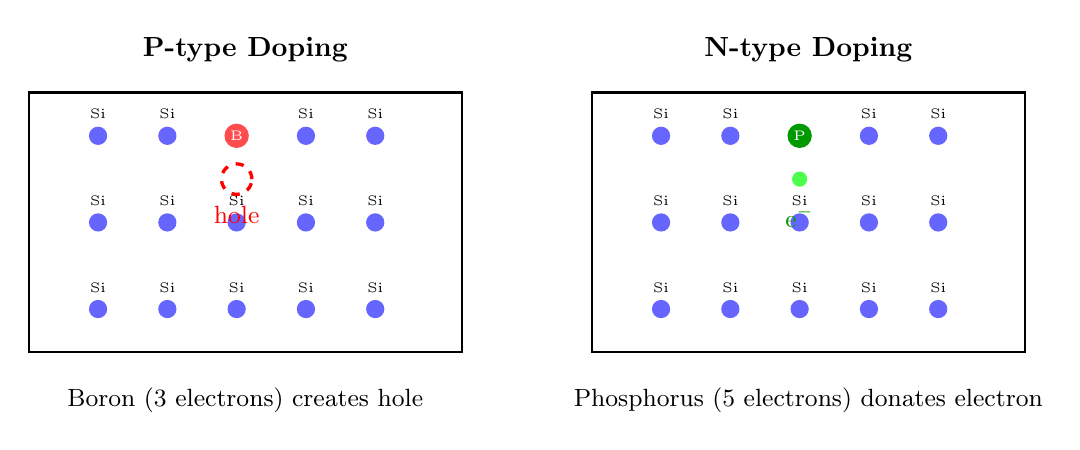
\begin{tikzpicture}[scale=1.1]
    % P-type doping
    \node[font=\bfseries] at (2.5,4) {P-type Doping};
    \draw[thick] (0,0.5) rectangle (5,3.5);

    % Si atoms
    \foreach \x/\y in {0.8/1, 1.6/1, 2.4/1, 3.2/1, 4/1, 0.8/2, 1.6/2, 2.4/2, 3.2/2, 4/2, 0.8/3, 1.6/3, 3.2/3, 4/3} {
        \fill[blue!60] (\x,\y) circle (3pt);
        \node[font=\tiny] at (\x,\y+0.25) {Si};
    }

    % Boron impurity
    \fill[red!70] (2.4,3) circle (4pt);
    \node[font=\tiny, white] at (2.4,3) {B};

    % Hole
    \draw[red, very thick, dashed] (2.4,2.5) circle (5pt);
    \node[below, red, font=\small] at (2.4,2.3) {hole};

    \node[below, font=\small] at (2.5,0.2) {Boron (3 electrons) creates hole};

    % N-type doping
    \node[font=\bfseries] at (9,4) {N-type Doping};
    \draw[thick] (6.5,0.5) rectangle (11.5,3.5);

    % Si atoms
    \foreach \x/\y in {7.3/1, 8.1/1, 8.9/1, 9.7/1, 10.5/1, 7.3/2, 8.1/2, 8.9/2, 9.7/2, 10.5/2, 7.3/3, 8.1/3, 9.7/3, 10.5/3} {
        \fill[blue!60] (\x,\y) circle (3pt);
        \node[font=\tiny] at (\x,\y+0.25) {Si};
    }

    % Phosphorus impurity
    \fill[green!60!black] (8.9,3) circle (4pt);
    \node[font=\tiny, white] at (8.9,3) {P};

    % Extra electron
    \fill[green!70] (8.9,2.5) circle (2.5pt);
    \node[below, green!60!black, font=\small] at (8.9,2.3) {e\(^-\)};

    \node[below, font=\small] at (9,0.2) {Phosphorus (5 electrons) donates electron};
\end{tikzpicture}
\caption{P-type and N-type Doping Process}
\end{figure}


\paragraph{Process:} Pentavalent impurity adds electrons (N-type), while Trivalent adds holes (P-type).
\paragraph{Mnemonic:}
\emph{``P-type: Positive holes from Trivalent; N-type: Negative electrons from Pentavalent''!}

% Q3(a) OR: Define RPV, PIV, Efficiency [3 marks]



\subsection{Question 3(a) OR [3 marks]}
\textbf{Define Ripple factor, Peak Inverse Voltage (PIV), Rectification efficiency.}

\subsubsection{Solution}

\paragraph{1. Ripple Factor (r):}
Ratio of RMS value of AC component to DC component in rectifier output.
\[
r = \frac{V_{ac(rms)}}{V_{dc}}
\]
Lower ripple factor indicates better filtering. Values: Half-wave = 1.21, Full-wave = 0.48.

\paragraph{2. Peak Inverse Voltage (PIV):}
Maximum reverse voltage across a diode when non-conducting. Diode must withstand this without breakdown. Values: Half-wave = \(V_m\), Full-wave center-tap = \(2V_m\), Bridge = \(V_m\).

\paragraph{3. Rectification Efficiency (\(\eta\)):}
Ratio of DC output power to AC input power.
\[
\eta = \frac{P_{dc}}{P_{ac}} \times 100\%
\]
Values: Half-wave = 40.6\%, Full-wave = 81.2\%.

\paragraph{Significance:} Low ripple factor is essential for audio circuits to prevent hum. PIV rating must be higher than peak voltage to avoid diode damage. Efficiency determines battery life in portable devices.

\paragraph{Mnemonic:}
\emph{``RPE: Ripple shows AC remaining, PIV protects diode, Efficiency measures conversion''!}

% Q3(b): Crystal Diode Working [3 marks]

\subsection{Question 3(b) [3 marks]}
\textbf{Explain working of Crystal diode.}

\subsubsection{Solution}

A \textbf{crystal diode} (PN junction diode) allows current flow in one direction only.

\paragraph{Construction:}
P-type and N-type semiconductors joined together form a PN junction with depletion region.

\paragraph{Working:}

\begin{description}
    \item[Forward Bias:] P-side connected to positive, N-side to negative. Barrier potential reduces, current flows when \(V > V_{\gamma}\) (0.7V for Si).

    \item[Reverse Bias:] P-side connected to negative, N-side to positive. Barrier increases, only tiny leakage current flows.
\end{description}

\paragraph{Applications:}
Rectification, clipping, clamping, voltage regulation.

\paragraph{Depletion Region:} The width of depletion region changes with applied voltage. It widens in reverse bias and narrows in forward bias, controlling current flow.


\paragraph{Biasing:} In forward bias the depletion layer decreases, in reverse bias it increases.
\paragraph{Mnemonic:}
\emph{``Crystal Clear: Forward flows, Reverse blocks''!}

% Q3(b) OR: Photodiode Working [3 marks]



\subsection{Question 3(b) OR [3 marks]}
\textbf{Explain working of photodiode.}

\subsubsection{Solution}

A \textbf{photodiode} converts light energy into electrical current, operating in reverse bias.

\paragraph{Working Principle:}
When photons strike the PN junction, they create electron-hole pairs. In reverse bias, these carriers are swept across junction by electric field, producing photocurrent proportional to light intensity.

\paragraph{Applications:}
Optical communication, light detection, solar cells, barcode readers.

\paragraph{Key Characteristic:} Photodiodes are always operated in reverse bias because the change in minority carrier current due to light is more significant and easier to measure than forward current changes.

\paragraph{Mnemonic:}
\emph{``Photodiode: Photons create current''!}

% Q3(c): Half-Wave Rectifier [4 marks] - WITH MANDATORY WAVEFORMS

\subsection{Question 3(c) [4 marks]}
\textbf{Explain half-wave rectifier with circuit diagram and waveforms.}

\subsubsection{Solution}

A \textbf{half-wave rectifier} converts AC to pulsating DC using a single diode, utilizing only one half-cycle of input.

\paragraph{Circuit Diagram:}

\begin{figure}[H]
\centering
\begin{circuitikz}[scale=1.1]
    % Transformer
    \draw (0,0) to[sV, l=\(V_{in}\)] (0,2);

    % Diode
    \draw (0,2) to[D, l=D] (3,2);

    % Load
    \draw (3,2) to[R, l=\(R_L\)] (3,0);

    % Ground
    \draw (0,0) -- (3,0);

    % Output
    \draw[<->] (3.5,2) -- (3.5,0) node[midway, right] {\(V_{out}\)};
\end{circuitikz}
\caption{Half-Wave Rectifier Circuit}
\end{figure}

\paragraph{Working:}
\textbf{Positive half-cycle:} Diode forward-biased, conducts. Output follows input.
\textbf{Negative half-cycle:} Diode reverse-biased, blocks. Output is zero.

\paragraph{Waveforms:}

\begin{figure}[H]
\centering
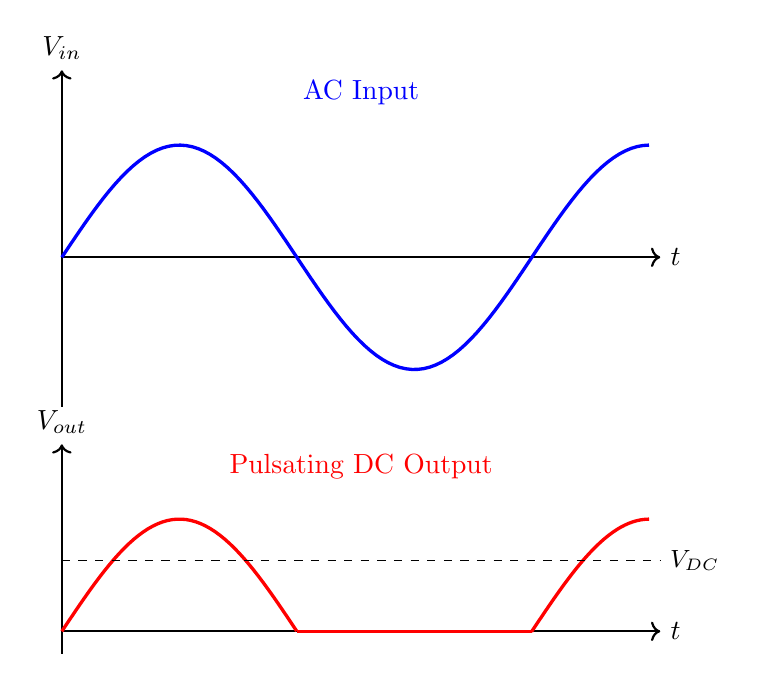
\begin{tikzpicture}[scale=0.95]
    % Input waveform
    \draw[->, thick] (0,0) -- (8,0) node[right] {\(t\)};
    \draw[->, thick] (0,-2) -- (0,2.5) node[above] {\(V_{in}\)};
    \draw[blue, very thick, domain=0:7.85, samples=100] plot (\x, {1.5*sin(\x r)});
    \node[blue]at (4,2.2) {AC Input};

    % Output waveform
    \begin{scope}[yshift=-5cm]
        \draw[->, thick] (0,0) -- (8,0) node[right] {\(t\)};
        \draw[->, thick] (0,-0.3) -- (0,2.5) node[above] {\(V_{out}\)};
        % Only positive half cycles
        \draw[red, very thick, domain=0:3.14, samples=50] plot (\x, {1.5*sin(\x r)});
        \draw[red, very thick] (3.14,0) -- (6.28,0);
        \draw[red, very thick, domain=6.28:7.85, samples=30] plot (\x, {1.5*sin(\x r)});
        \node[red] at (4,2.2) {Pulsating DC Output};
        \draw[dashed] (0,0.95) -- (8,0.95) node[right, font=\small] {\(V_{DC}\)};
    \end{scope}
\end{tikzpicture}
\caption{Half-Wave Rectifier Waveforms}
\end{figure}

\paragraph{Specifications:}
\begin{itemize}
    \item DC Output: \(V_{DC} = \frac{V_m}{\pi} = 0.318 V_m\)
    \item Efficiency: \(\eta = 40.6\%\)
    \item Ripple Factor: \(r = 1.21\)
    \item PIV: \(V_m\)
\end{itemize}


\paragraph{Filter:} A filter circuit is needed to make the rectifier output smooth DC.
\paragraph{Mnemonic:}
\emph{``Half-wave uses Half the cycle''!}

% Q3(c) OR: Full-Wave Rectifier [4 marks] - WITH MANDATORY WAVEFORMS



\subsection{Question 3(c) OR [4 marks]}
\textbf{Explain full-wave rectifier with circuit diagram and waveforms.}

\subsubsection{Solution}

A \textbf{full-wave rectifier} converts AC to pulsating DC using both half-cycles, with center-tapped transformer and two diodes.

\paragraph{Circuit Diagram:}

\begin{figure}[H]
\centering
\begin{circuitikz}[scale=1.0]
    % Transformer with center tap
    \draw (0,0) to[sV] (0,3);
    \draw (0,3) -- (1,3) -- (1,3.5) node[above] {A};
    \draw (0,1.5) -- (1,1.5) node[right] {CT};
    \draw (0,0) -- (1,0) -- (1,-0.5) node[below] {B};

    % Diodes
    \draw (1,3.5) to[D, l=\(D_1\)] (3.5,3.5);
    \draw (1,-0.5) to[D, l=\(D_2\)] (3.5,-0.5);

    % Load
    \draw (3.5,3.5) -- (3.5,2.5);
    \draw (3.5,2.5) to[R, l=\(R_L\)] (3.5,0.5);
    \draw (3.5,0.5) -- (3.5,-0.5);

    % Center tap to ground
    \draw (1,1.5) -- (3.5,1.5);
    \draw (2.25,1.5) node[ground]{};

    % Output
    \draw[<->] (4,2.5) -- (4,0.5) node[midway, right] {\(V_{out}\)};
\end{circuitikz}
\caption{Full-Wave Rectifier (Center-Tap) Circuit}
\end{figure}

\paragraph{Working:}
\textbf{Positive half:} A positive, B negative. \(D_1\) conducts, \(D_2\) blocks.
\textbf{Negative half:} B positive, A negative. \(D_2\) conducts, \(D_1\) blocks.
Both halves produce output in same direction through load.

\paragraph{Waveforms:}

\begin{figure}[H]
\centering
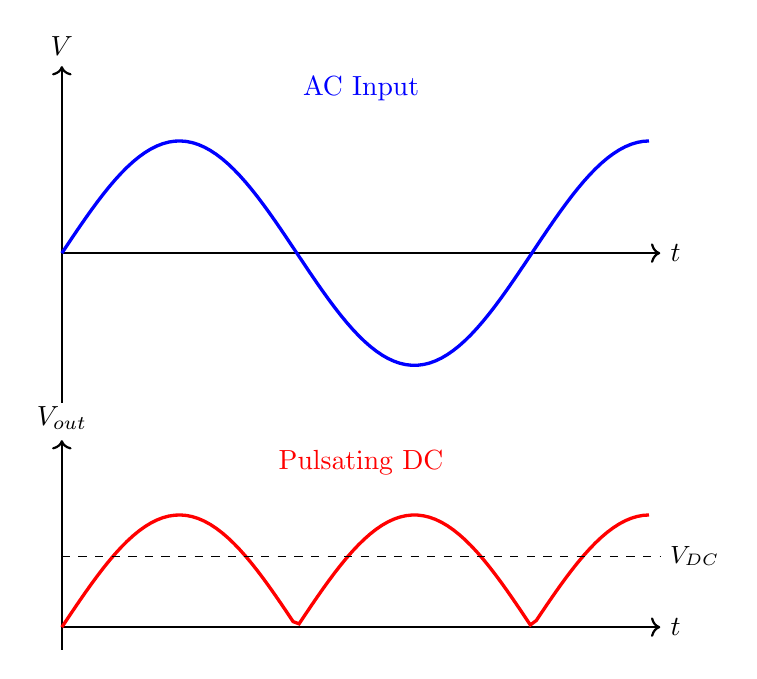
\begin{tikzpicture}[scale=0.95]
    % Input
    \draw[->, thick] (0,0) -- (8,0) node[right] {\(t\)};
    \draw[->, thick] (0,-2) -- (0,2.5) node[above] {\(V\)};
    \draw[blue, very thick, domain=0:7.85, samples=100] plot (\x, {1.5*sin(\x r)});
    \node[blue] at (4,2.2) {AC Input};

    % Output
    \begin{scope}[yshift=-5cm]
        \draw[->, thick] (0,0) -- (8,0) node[right] {\(t\)};
        \draw[->, thick] (0,-0.3) -- (0,2.5) node[above] {\(V_{out}\)};
        \draw[red, very thick, domain=0:7.85, samples=100] plot (\x, {1.5*abs(sin(\x r))});
        \node[red] at (4,2.2) {Pulsating DC};
        \draw[dashed] (0,0.95) -- (8,0.95) node[right, font=\small] {\(V_{DC}\)};
    \end{scope}
\end{tikzpicture}
\caption{Full-Wave Rectifier Waveforms}
\end{figure}

\paragraph{Specifications:}
\begin{itemize}
    \item DC Output: \(V_{DC} = \frac{2V_m}{\pi} = 0.636 V_m\)
    \item Efficiency: \(\eta = 81.2\%\)
    \item Ripple Factor: \(r = 0.48\)
    \item PIV: \(2V_m\)
    \item Ripple Frequency: \(2f\) (double input frequency)
\end{itemize}

\paragraph{Mnemonic:}
\emph{``Full-wave uses Full cycle, double efficiency''!}

% Q3(d): VI Characteristics of PN Diode [4 marks]

\subsection{Question 3(d) [4 marks]}
\textbf{Draw and explain VI characteristics of PN junction diode.}

\subsubsection{Solution}

The \textbf{Voltage-Current (VI) characteristic} shows the relationship between voltage and current in a PN diode.

\begin{figure}[H]
\centering
\begin{tikzpicture}[scale=1.1]
    % Axes
    \draw[->, very thick] (-4,0) -- (4,0) node[right] {\(V\) (Voltage)};
    \draw[->, very thick] (0,-2.5) -- (0,3.5) node[above] {\(I\) (Current)};

    % Forward characteristic
    \draw[blue, very thick, domain=0.6:3.5, samples=50] plot (\x, {3*(\x-0.5)^2});

    % Reverse characteristic
    \draw[red, very thick] (-3.5,-0.4) -- (-0.1,-0.4);

    % Breakdown
    \draw[red, very thick] (-3.5,-0.4) -- (-3.5,-2.3);

    % Labels
    \node[blue] at (2.5,3.2) {Forward Bias};
    \node[red] at (-2.5,-0.7) {Reverse Bias};
    \node[red] at (-3,-2.3) {Breakdown};

    % Key points
    \draw[dashed] (0.7,0) -- (0.7,0.5);
    \node[below] at (0.7,-0.2) {\(V_{\gamma}\)};
    \node[below, font=\tiny] at (0.7,-0.5) {0.7V (Si)};

    \draw[dashed] (0,-0.4) -- (-1,-0.4);
    \node[left, font=\small] at (-0.2,-0.4) {\(-I_S\)};

    \draw[dashed] (-3.5,0) -- (-3.5,-0.4);
    \node[above, font=\small] at (-3.5,0.2) {\(V_{BR}\)};
\end{tikzpicture}
\caption{VI Characteristics of PN Junction Diode}
\end{figure}

\paragraph{Regions:}

\begin{description}
    \item[Forward Bias (\(V > 0\)):] Small current until \(V_{\gamma}\) (knee voltage). Beyond threshold, current increases exponentially.

    \item[Reverse Bias (\(V < 0\)):] Small reverse saturation current \(I_S\) (few \(\mu\)A) due to minority carriers. Nearly constant.

    \item[Breakdown (\(V < V_{BR}\)):] At large reverse voltage, avalanche/Zener breakdown occurs. Current increases rapidly.
\end{description}


\paragraph{Knee Voltage:} It is 0.7V for Si diode and 0.3V for Ge diode.
\paragraph{Mnemonic:}
\emph{``Forward flows after threshold; Reverse resists except breakdown''!}

% Q3(d) OR: P-type vs N-type [4 marks]



\subsection{Question 3(d) OR [4 marks]}
\textbf{Write difference between P-type and N-type semiconductor.}

\subsubsection{Solution}

\begin{table}[H]
\centering
\caption{P-type vs N-type Semiconductor}
\begin{tabularx}{\textwidth}{lXX}
\toprule
\textbf{Parameter} & \textbf{P-type} & \textbf{N-type} \\
\midrule
Doping & Trivalent (B, Ga, In) & Pentavalent (P, As, Sb) \\
Majority Carriers & Holes (\(h^+\)) & Electrons (\(e^-\)) \\
Minority Carriers & Electrons & Holes \\
Donor/Acceptor & Acceptor atoms & Donor atoms \\
Conductivity & Hole conduction & Electron conduction \\
Fermi Level & Near valence band & Near conduction band \\
\bottomrule
\end{tabularx}
\end{table}

\paragraph{Energy Levels:} In N-type, donor energy level is very close to the conduction band (0.01eV for Ge). In P-type, acceptor energy level is near the valence band. This requires less energy for ionization.

\paragraph{Conductivity:} In N-type, conductivity is predominantly due to electrons which have higher mobility than holes. Hence N-type devices are generally faster than P-type devices.

\paragraph{Mnemonic:}
\emph{``P for Positive holes; N for Negative electrons''!}

% ========================================
% QUESTION 4: Diodes & Regulators (14 marks)
% ========================================

\section{Question 4}

% This section covers special diodes and voltage regulation.

% Q4(a): LED Principle [3 marks]


\subsection{Question 4(a) [3 marks]}
\textbf{Explain the principle of operation of LED.}

\subsubsection{Solution}

A \textbf{Light Emitting Diode (LED)} converts electrical energy into light through \textbf{electroluminescence}.

\paragraph{Principle:}
When forward current flows, electrons from N-region recombine with holes in P-region at the junction. Energy is released as photons (light). The wavelength (color) depends on the semiconductor band gap energy.

\paragraph{Energy Relationship:}
\[
E = h\nu = \frac{hc}{\lambda} = E_g
\]
where \(E_g\) is band gap energy, determining color.

\paragraph{Materials \& Colors:}
GaAs (Red), GaP (Green), GaN (Blue), InGaN (White).

\paragraph{Material Selection:} Silicon and Germanium are not used for LEDs because they release energy as heat (indirect bandgap). Gallium Arsenide/Phosphide are direct bandgap materials used for light emission.


\paragraph{Voltage:} For a red LED, the forward voltage is typically 1.8V.
\paragraph{Mnemonic:}
\emph{``LED: Light from Energy Drop during recombination''!}

% Q4(a) OR: LED Applications [3 marks]

\subsection{Question 4(a) OR [3 marks]}
\textbf{State applications of LED.}

\subsubsection{Solution}

\paragraph{Applications:}
\begin{enumerate}
    \item Display panels (seven-segment, dot-matrix)
    \item Indicator lights (power, status)
    \item Traffic signals
    \item Automotive lighting
    \item General illumination
    \item Backlighting (LCD screens)
    \item Optical communication
\end{enumerate}

\paragraph{Advantages:} LEDs consume very low power compared to incandescent bulbs, have longer life span (>50,000 hours), faster switching speed (ns), and high mechanical ruggedness.

\paragraph{Efficiency:} LEDs convert about 80-90% of energy into light, whereas incandescent bulbs convert only 10-20%, wasting the rest as heat. This makes LEDs highly energy-efficient.

\paragraph{Industrial Use:} In automated industries, LEDs are used in sensor systems, quality control scanners, and machine vision lighting due to their reliability and consistent spectral output.

\paragraph{Mnemonic:}
\emph{``LED everywhere: Displays, Indicators, Traffic, Automotive''!}

% Q4(b): Zener as Voltage Regulator [4 marks]

\subsection{Question 4(b) [4 marks]}
\textbf{Explain Zener diode as voltage regulator.}

\subsubsection{Solution}

A \textbf{Zener diode} maintains constant output voltage by operating in reverse breakdown region.

\paragraph{Circuit:}

\begin{figure}[H]
\centering
\begin{circuitikz}[scale=1.2]
    % Input
    \draw (0,0) to[V, l=\(V_{in}\)] (0,3);

    % Series resistor
    \draw (0,3) to[R, l=\(R_S\)] (3,3);

    % Zener diode
    \draw (3,3) to[zzD, l=\(V_Z\)] (3,0);

    % Load
    \draw (3,3) -- (5,3);
    \draw (5,3) to[R, l=\(R_L\)] (5,0);

    % Ground
    \draw (0,0) -- (5,0);

    % Output
    \draw[<->] (5.5,3) -- (5.5,0) node[midway, right] {\(V_{out}=V_Z\)};
\end{circuitikz}
\caption{Zener Voltage Regulator}
\end{figure}

\paragraph{Working:}
\(R_S\) drops excess voltage. Zener maintains \(V_{out} = V_Z\). Changes in \(V_{in}\) or \(I_L\) are absorbed by varying \(I_Z\).

\[
I_S = I_Z + I_L = \frac{V_{in} - V_Z}{R_S}
\]

\paragraph{Design Condition:} For proper regulation, the Zener diode must remain in breakdown region. The current through Zener (\(I_Z\)) must be between \(I_{Z(\text{min})}\) and \(I_{Z(\text{max})}\) under all load conditions.

\paragraph{Regulation Factor:} The quality of regulation is measured by line regulation (input change) and load regulation (load change). Zener provides acceptable regulation for low cost applications.


\paragraph{Doping:} The doping level in a Zener diode is much higher than in a normal diode.
\paragraph{Mnemonic:}
\emph{``Zener Zaps excess, maintains constant voltage''!}

% Q4(b) OR: Zener Limitations [4 marks]

\subsection{Question 4(b) OR [4 marks]}
\textbf{Give limitations of zener voltage regulator.}

\subsubsection{Solution}

\paragraph{Limitations:}
\begin{enumerate}
    \item Limited current capacity (few mA to few A)
    \item Poor efficiency (power dissipated as heat)
    \item Output voltage not adjustable (fixed by Zener)
    \item Limited ripple rejection
    \item Not suitable for high power applications
    \item Requires minimum load current
\end{enumerate}

\paragraph{Temperature Dependence:} Zener voltage changes with temperature. Zener breakdown has negative temperature coefficient, while Avalanche breakdown has positive coefficient. This can affect stability in precision circuits.

\paragraph{Noise:} Zener diodes generate significant noise in the avalanche breakdown region. This noise can interfere with sensitive signal processing circuits, requiring additional bypass capacitors.

\paragraph{Stability:} For very high precision voltage references, standard Zener diodes are often replaced by bandgap reference circuits which offer much better temperature stability and lower noise performance.

\paragraph{Mnemonic:}
\emph{``Zener limits: Low current, Fixed voltage, Heat loss''!}

% Q4(c): Filter Circuit Necessity [7 marks]

\subsection{Question 4(c) [7 marks]}
\textbf{Discuss the necessity of filter circuit in rectifier. List various types of filter circuits used in rectifier and explain any one with neat diagram.}

\subsubsection{Solution}

\paragraph{Necessity of Filter Circuit:}

Rectifier output is pulsating DC with significant AC ripple. Filters smooth this into steady DC for:
\begin{itemize}
    \item Protecting sensitive electronic components
    \item Reducing ripple factor
    \item Improving voltage regulation
    \item Minimizing electrical noise
\end{itemize}

\paragraph{Types of Filter Circuits:}
\begin{enumerate}
    \item Capacitor filter (C)
    \item Inductor filter (L)
    \item LC filter
    \item CLC filter (\(\pi\)-filter)
    \item RC filter
\end{enumerate}

\paragraph{Explanation: Capacitor Filter}

\subparagraph{Circuit:}

\begin{figure}[H]
\centering
\begin{circuitikz}[scale=1.0]
    % Rectifier
    \draw (0,0) to[sV] (0,2);
    \draw (0,2) to[D] (2,2);

    % Capacitor
    \draw (2,2) to[short] (3,2);
    \draw (3,2) to[C, l=\(C\)] (3,0);

    % Load
    \draw (3,2) to[short] (4.5,2);
    \draw (4.5,2) to[R, l=\(R_L\)] (4.5,0);

    % Ground
    \draw (0,0) -- (4.5,0);

    % Output
    \draw[<->] (5,2) -- (5,0) node[midway, right] {\(V_{out}\)};
\end{circuitikz}
\caption{Capacitor Filter Circuit}
\end{figure}

\subparagraph{Working:}
Capacitor charges to peak during conduction, discharges through load when diode is OFF. Provides relatively smooth DC with small ripple.

\subparagraph{Waveform:}

\begin{figure}[H]
\centering
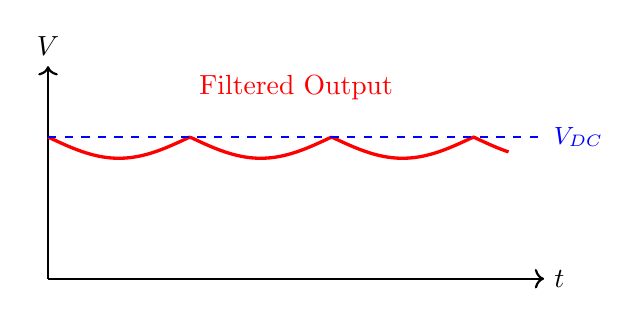
\begin{tikzpicture}[scale=0.9]
    \draw[->, thick] (0,0) -- (7,0) node[right] {\(t\)};
    \draw[->, thick] (0,0) -- (0,3) node[above] {\(V\)};

    % Ripple waveform
    \draw[red, very thick, domain=0:6.5, samples=200] plot (\x, {2 - 0.3*abs(sin(1.57*\x r))});
    \node[red] at (3.5,2.7) {Filtered Output};

    \draw[dashed, blue] (0,2) -- (7,2) node[right, font=\small] {\(V_{DC}\)};
\end{tikzpicture}
\caption{Capacitor Filter Output Waveform}
\end{figure}

\subparagraph{Specifications:}
Ripple: \(V_{ripple} \approx \frac{I_{DC}}{fC}\)
Good for low current loads.

\paragraph{Comparison:} L-filter is good for heavy loads/low resistance. C-filter is good for light loads/high resistance. Pi-filter provides best smoothing but is bulky. Selection depends on load and cost constraints.


\paragraph{Additional Info:} Without filter circuits, noise (hum) occurs in electronic devices. A combination of capacitor and inductor gives the best filtering.
\paragraph{Mnemonic:}
\emph{``Filter Flattens pulsating DC to smooth DC''!}

% ========================================
% QUESTION 5: Environmental & Transistors (14 marks)
% ========================================

\section{Question 5}

% This section covers environmental issues and transistor applications.

% Q5(a): E-waste Definition [3 marks]


\subsection{Question 5(a) [3 marks]}
\textbf{Define e-waste. List common e-waste items.}

\subsubsection{Solution}

\paragraph{Definition:}
\textbf{E-waste (Electronic Waste)} refers to discarded electrical or electronic devices and their components. It includes obsolete, broken, or end-of-life electronic products.

\paragraph{Common E-waste Items:}
\begin{itemize}
    \item Computers, laptops, tablets
    \item Mobile phones, chargers
    \item TVs, monitors
    \item Printers, scanners
    \item Batteries (lithium, lead-acid)
    \item Circuit boards, cables
    \item Home appliances (refrigerators, washing machines)
\end{itemize}

\paragraph{Environmental Impact:} E-waste usually contains hazardous substances like Lead (Pb), Cadmium (Cd), Mercury (Hg), and Brominated Flame Retardants (BFR) which contaminate soil and water if dumped.

\paragraph{Sources:} Major sources include IT equipment (servers, PCs), consumer electronics (TVs, cameras), large household appliances, and toys. Rapid technology upgrades increase waste volume.


\paragraph{Warning:} E-waste should not be thrown with normal trash. Toxic substances in it need to be recycled.
\paragraph{Mnemonic:}
\emph{``E-waste: Electronics discarded after use''!}

% Q5(b): E-waste Management [3 marks]

\subsection{Question 5(b) [3 marks]}
\textbf{State and explain various strategies of e-waste management.}

\subsubsection{Solution}

\paragraph{E-waste Management Strategies:}

\begin{description}
    \item[Reduce:] Extend product lifespan through repair and maintenance. Buy durable products.

    \item[Reuse:] Donate or sell working devices. Repurpose components.

    \item[Recycle:] Extract valuable materials (gold, copper, rare metals) through proper recycling facilities.

    \item[Proper Disposal:] Use authorized e-waste collection centers. Never dump in landfills.

    \item[Awareness:] Educate public about hazards and proper disposal methods.
\end{description}

\paragraph{Legislation:} Governments implement EPR (Extended Producer Responsibility) laws, making manufacturers responsible for the entire lifecycle of electronic products, encouraging eco-friendly design.


\paragraph{Benefit:} Precious metals like gold, silver, and copper can be recovered from E-waste recycling.
\paragraph{Mnemonic:}
\emph{``3R+: Reduce, Reuse, Recycle, Right disposal''!}

% Q5(c): Transistor as Switch [4 marks]

\subsection{Question 5(c) [4 marks]}
\textbf{Explain transistor as switch.}

\subsubsection{Solution}

A transistor operates as an electronic switch with two states: ON (saturation) and OFF (cutoff).

\paragraph{Circuit:}

\begin{figure}[H]
\centering
\begin{circuitikz}[scale=1.1]
    % Supply
    \draw (0,4) to[V, l=\(V_{CC}\)] (0,0);

    % Load resistor
    \draw (0,4) to[R, l=\(R_C\)] (3,4);

    % Transistor
    \draw (3,2) node[npn](npn1){};
    \draw (npn1.C) -- (3,4);
    \draw (npn1.E) -- (3,0);

    % Base resistor
    \draw (0,2) to[R, l=\(R_B\)] (npn1.B);
    \draw (0,2) to[short] (-1,2) node[left] {\(V_{in}\)};

    % Ground
    \draw (0,0) -- (3,0);

    % Output
    \draw (3,4) to[short] (4,4) node[right] {\(V_{out}\)};
\end{circuitikz}
\caption{Transistor as Switch}
\end{figure}

\paragraph{States:}

\begin{description}
    \item[OFF (Cutoff):] \(V_{in} = 0V\), base current \(I_B = 0\), \(I_C \approx 0\), \(V_{out} = V_{CC}\) (Switch OPEN)

    \item[ON (Saturation):] \(V_{in} = High\), \(I_B\) sufficient, \(I_C = I_{C(sat)}\), \(V_{out} \approx 0V\) (Switch CLOSED)
\end{description}

\paragraph{Applications:}
Digital circuits, relay drivers, LED drivers, motor control.

\paragraph{Ideal vs Real:} Ideally, a switch has zero resistance when ON and infinite when OFF. Transistors have small saturation voltage (\(V_{CE(sat)} \approx 0.2V\)) when ON and small leakage current when OFF.


\paragraph{State:} In saturation region transistor acts as ON switch and in cut-off as OFF switch.
\paragraph{Mnemonic:}
\emph{``Transistor Switch: Base controls Collector current''!}

% Q5(d): Alpha-Beta Relation [4 marks]

\subsection{Question 5(d) [4 marks]}
\textbf{Derive relation between \(\alpha\) and \(\beta\) for CE configuration of transistor.}

\subsubsection{Solution}

For a transistor in Common Emitter configuration:

\paragraph{Definitions:}
\[
\alpha = \frac{I_C}{I_E} \quad (\text{Common Base gain})
\]
\[
\beta = \frac{I_C}{I_B} \quad (\text{Common Emitter gain})
\]

\paragraph{Derivation:}

From Kirchhoff's Current Law:
\[
I_E = I_B + I_C
\]

From definition of \(\alpha\):
\[
I_C = \alpha I_E = \alpha(I_B + I_C)
\]

Expanding:
\[
I_C = \alpha I_B + \alpha I_C
\]

Rearranging:
\[
I_C(1 - \alpha) = \alpha I_B
\]

\[
\frac{I_C}{I_B} = \frac{\alpha}{1-\alpha}
\]

Since \(\beta = \frac{I_C}{I_B}\):

\[
\boxed{\beta = \frac{\alpha}{1-\alpha}}
\]

Similarly, solving for \(\alpha\):

\[
\boxed{\alpha = \frac{\beta}{1+\beta}}
\]

\paragraph{Example:}
If \(\alpha = 0.98\): \(\beta = \frac{0.98}{1-0.98} = 49\)

If \(\beta = 100\): \(\alpha = \frac{100}{1+100} = 0.99\)

\paragraph{Significance:} Value of \(\alpha\) is always slightly less than 1 (0.95 to 0.99) as \(I_C < I_E\). Value of \(\beta\) is much greater than 1 (typically 50-300), showing high current gain capability of CE configuration.

\paragraph{Application:} High beta allows transistors to act as amplifiers. A small base current variation causes a large collector current variation, amplifying the input signal.


\paragraph{Remember:} Always \(\beta > \alpha\). The value of \(\alpha\) is close to 1, while \(\beta\) can be from 20 to 500.
\paragraph{Mnemonic:}
\emph{``Alpha over one-minus-alpha equals Beta''!}

\end{document}

